%______________________________________________________
%
%   LaTeX-mall fr nybrjare
%
%   Konstruerad av Marcus Bergner, bergner@cs.umu.se
%
%   Vid funderingar titta lngst ned i denna fil,
%   eller skicka ett mail
%______________________________________________________
%

% lite instllningar
\documentclass[10pt, titlepage, oneside, a4paper]{article}
\usepackage{amsmath}
\usepackage[T1]{fontenc}
\usepackage[utf8]{inputenc}
\usepackage[english]{babel}
\usepackage{amssymb, graphicx, fancyheadings}
\usepackage{placeins}

%For subfigures
\usepackage{caption}
\usepackage{subcaption}
%For including matlab code
%\usepackage{mcode}

\addtolength{\textheight}{20mm}
\addtolength{\voffset}{-5mm}
\renewcommand{\sectionmark}[1]{\markleft{#1}}

% \Section ger mindre spillutrymme, anvnd dem om du vill
\newcommand{\Section}[1]{\section{#1}\vspace{-8pt}}
\newcommand{\Subsection}[1]{\vspace{-4pt}\subsection{#1}\vspace{-8pt}}
\newcommand{\Subsubsection}[1]{\vspace{-4pt}\subsub\section{#1}\vspace{-8pt}}
	
% appendices, \appitem och \appsubitem r fr bilagor
\newcounter{appendixpage}

\newenvironment{appendices}{
	\setcounter{appendixpage}{\arabic{page}}
	\stepcounter{appendixpage}
}{
}

\newcommand{\appitem}[2]{
	\stepcounter{section}
	\addtocontents{toc}{\protect\contentsline{section}{\numberline{\Alph{section}}#1}{\arabic{appendixpage}}}
	\addtocounter{appendixpage}{#2}
}

\newcommand{\appsubitem}[2]{
	\stepcounter{subsection}
	\addtocontents{toc}{\protect\contentsline{subsection}{\numberline{\Alph{section}.\arabic{subsection}}#1}{\arabic{appendixpage}}}
	\addtocounter{appendixpage}{#2}
}

% ndra de rader som behver ndras
%\def\inst{Department of computer science}
\def\inst{Department of Mathematics and Mathematical Statistics}
\def\typeofdoc{Lab report}
\def\course{Numerical methods for PDE 7.5hp}
\def\pretitle{Laboratory 2}
\def\title{Hyperbolic Equations}
\def\name{Robin Lundberg}
\def\username{rolu0008}
\def\email{\username{}@student.umu.se}
\def\path{}
\def\graders{Patrik Norqvist, Christian Engström and Juan Carlos Araujo-Cabarcas.}


% om du vill referera till katalogen dr dina filer ligger kan du 
% anvnda \fullpath som kommer att vara "~username/edu..." o.s.v.
%\def\fullpath{\raisebox{1pt}{$\scriptstyle \sim$}\username/\path}


% Hr brjar sjlva dokumentet
\begin{document}

	% skapar framsidan (om den inte duger: gr helt enkelt en egen)
	\begin{titlepage}
		\thispagestyle{empty}
		\begin{large}
			\begin{tabular}{@{}p{\textwidth}@{}}
				\textbf{UMEÅ UNIVERSITY \hfill \today} \\
				\textbf{\inst} \\
				\textbf{\typeofdoc} \\
			\end{tabular}
		\end{large}
		\vspace{10mm}
		\begin{center}
			\LARGE{\pretitle} \\
			\huge{\textbf{\course}}\\
			\vspace{10mm}
			\LARGE{\title} \\
			\vspace{15mm}
			\begin{large}
				\begin{tabular}{ll}
					\textbf{Name} & \name \\
					\textbf{E-mail} & \texttt{\email} \\
					%\textbf{Path} & \texttt{/home/rolund03/workspace/gsl\_ode} \\
				\end{tabular}
			\end{large}
			\vfill
			\large{\textbf{Supervisor}}\\
			\mbox{\large{\graders}}
		\end{center}
	\end{titlepage}


	% fixar sidfot
	\lfoot{\footnotesize{\name, \email}}
	\rfoot{\footnotesize{\today}}
	\lhead{\sc\footnotesize\title}
	\rhead{\nouppercase{\sc\footnotesize\leftmark}}
	\pagestyle{fancy}
	\renewcommand{\headrulewidth}{0.2pt}
	\renewcommand{\footrulewidth}{0.2pt}

	% skapar innehllsfrteckning.
	% Tnk p att kra latex 2ggr fr att uppdatera allt
	\pagenumbering{roman}
	%\tableofcontents
	
	% och lägger in en sidbrytning
	\newpage

	\pagenumbering{arabic}

	% i Sverige har vi normalt inget indrag vid nytt stycke
	\setlength{\parindent}{0pt}
	% men dremot lite mellanrum
	\setlength{\parskip}{10pt}

	% lägger in rubrik (finns \section, men då får man mycket spillutrymme)
	\FloatBarrier
	\Section{Theory}
	In this lab I used five different methods to solve the one dimensional wave equation
\begin{equation}\label{eq:wave}
	\frac{\partial^2 u}{\partial t^2} = c^2 \frac{\partial^2 u}{\partial x^2}, \qquad 0\le x \le L
\end{equation}
where $c$ is the propagation speed of the wave, $u=u(x,t)$ is the displacement from equilibrium.
The initial and boundary conditions to be solved for are
\begin{equation}\label{eq:initial}
\begin{aligned}%{rcl}
	u(0,t) & = u(L,t) = 0 \\
	u(x,0) & = f(x) \\
	\dot{u}(x,0) & = 0
\end{aligned}
\end{equation}
where $f(x)$ is a known function.

From now on we discretize $u$ in both time, $t$, and space, $x$. So that
\begin{equation}
\begin{aligned}
	u(j \Delta x, n \Delta t) = u_j^n \\
	j = 0, 1, \dots, J=10/\Delta x \\
	n = 0, 1, \dots, N=T/\Delta t \\
\end{aligned}
\end{equation}
where $\Delta x$ and $\Delta t$ are constants chosen so that $N$ and $J$ are integers.

\subsection{Simple Explicit Method}\label{sec:explicit}
This method is also known as \emph{Forward in time, centred in space} (FTCS).
Eq. \eqref{eq:wave} can be rewritten in discretized form as
\begin{equation}
\frac{u_{j}^{n+1} - 2 u_{j}^{n} + u_{j}^{n-1}}{\Delta t^2} = c^2 \frac{u_{j+1}^{n} - 2 u_{j}^{n} + u_{j-1}^{n}}{\Delta x^2}.
\end{equation}
Solving this for $u_{j}^{n+1}$ gives the updating scheme.
%\begin{equation}
%u_{j}^{n+1} = 2 u_{j}^{n} - u_{j}^{n-1} + \frac{c^2\Delta t^2}{\Delta x^2} \left( u_{j+1}^{n} - 2 u_{j}^{n} + u_{j-1}^{n} \right).
%\end{equation}


\subsection{Fully Implicit Method}\label{sec:implicit}
For the implicit method we discretize eq. \eqref{eq:wave} having the spacial derivative calculated forward in time like
\begin{equation}\label{eq:implicit}
\frac{u_{j}^{n+1} - 2 u_{j}^{n} + u_{j}^{n-1}}{\Delta t^2} = c^2 \frac{u_{j+1}^{n+1} - 2 u_{j}^{n+1} + u_{j-1}^{n+1}}{\Delta x^2}.
\end{equation}
Solving this for $u_{j}^{n+1}$ gives the updating scheme.
%\begin{equation}
%u_{j}^{n+1} \left(1 + \frac{c^2\Delta t^2}{\Delta x^2}\right) - \frac{1}{2}\frac{c^2\Delta t^2}{\Delta x^2} \left[ u_{j+1}^{n+1}+u_{j-1}^{n+1} \right] = 2 u_{j}^{n} - u_{j}^{n-1}.
%\end{equation}


\subsection{The Crank-Nicholson Method}\label{sec:crank}
The \emph{Crank-Nicholson} method is similar to the implicit method except that the average in time in both LHS and RHS of eq. \eqref{eq:implicit} should be the same. In order to accomplish this, take the average of the spacial derivative forwards and backwards in time. So that 
\begin{equation}\label{eq:crank}
\frac{u_{j}^{n+1} - 2 u_{j}^{n} + u_{j}^{n-1}}{\Delta t^2} = \frac{c^2}{2} 
\frac{(u_{j+1}^{n+1}+u_{j+1}^{n-1}) - 2 (u_{j}^{n+1}+u_{j}^{n-1}) + (u_{j-1}^{n+1}+u_{j-1}^{n-1})}{\Delta x^2}.
\end{equation}
Solving this for $u_{j}^{n+1}$ gives the updating scheme.
%\begin{equation}
%u_{j}^{n+1} \left(1 + \frac{c^2\Delta t^2}{\Delta x^2}\right) - \frac{1}{2}\frac{c^2\Delta t^2}{\Delta x^2} \left[ u_{j+1}^{n+1}+u_{j-1}^{n+1} \right] = 2 u_{j}^{n} - u_{j}^{n-1}.
%\end{equation}


\subsection{FFT Time-step Method in Normal Space}\label{sec:ffttime}
The updating scheme for this problem was derived in \cite{FDNotes} for time-stepping in 
normal space.

\subsection{Immediate FFT Method}\label{sec:fftimm}
The numerical solution for this method was derived in \cite{FDNotes}.





	
	\FloatBarrier
	\Section{Results}
	\subsection{\label{}Oscillation of the tuning fork}

A tuning fork is an acoustic resonator in the shape of a fork with two prongs, forming a U. it is usually made of elastic metal, as f.i. Steel. Apart from the fundamental mode, as illustrated in \ref{fig:tuning}, the tuning fork can also oscillate in higher overtones. Due to the fact, that these higher modes are damped more strongly by the base, they die out faster and leave a a typical pure musical tone. This also causes the short “clang”, that appears when tipping the fork. The pitch of a particular tuning fork depends on the length as well as on the mass of the prongs.

\begin{figure}[H]
	\centering
	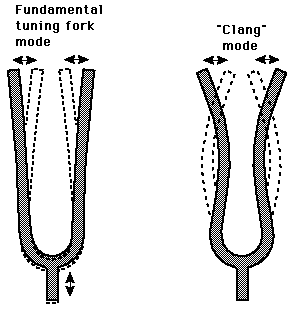
\includegraphics[angle=0,width=0.6\textwidth]{img/tuning}
	\caption{First two balanced modes of a tuning fork.}
	\label{fig:tuning}
\end{figure}

Apart from the modes in which the two prongs oscillate in antiphase, of which the two first are shown in \ref{fig:tuning}, more unbalanced modes exist that transfer onto the base. As the base is in general fixed by holding the tuning fork in the hand or having it fixed by other means, these modes generally don't appear significantly.
The main interest was to measure amplitude and frequency of the vibrations of the tuning fork. To do so, the difference and the sum of the two currents as given out by the electric circuit explained in \ref{} were processed with labview. To calibrate the PSD, the micrometer screw attached to the slide of the tuning fork was used.

In \ref{fig:frequency} the vibration of the tuning fork after 3 seconds of damping is illustrated. The difference of the two currents, that the PSD feeds the electric circuit with, is depicted as a function of the time. As can be seen the tuning fork is harmonically oscillating at a steady frequency.

\begin{figure}[H]
	\centering
	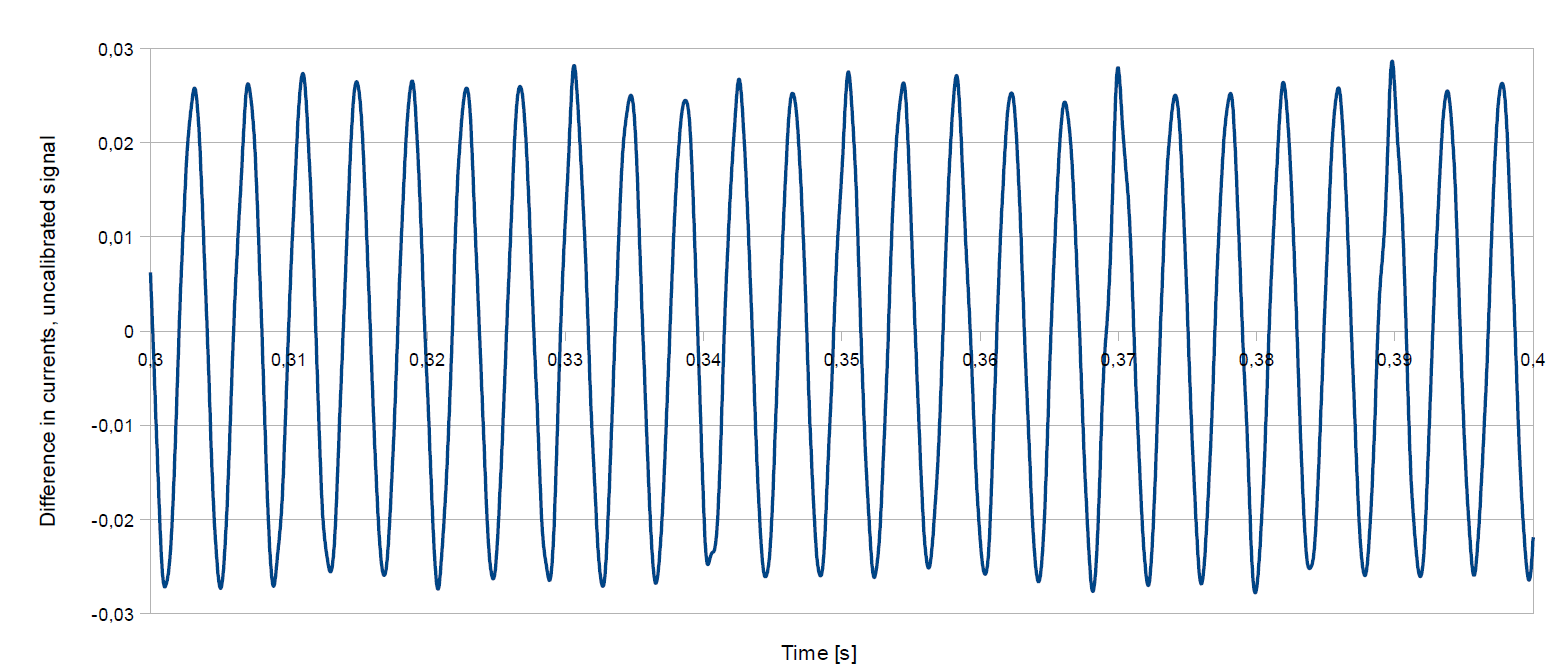
\includegraphics[angle=0,width=0.6\textwidth]{img/frequency}
	\caption{Uncalibrated difference in currents given out by the PSD.}
	\label{fig:frequency}
\end{figure}

This frequency was determined by averaging the periodic time $T$ over 229 periods. Doing this, a frequency of 

\begin{eqnarray}
f = 253,68 Hz
\end{eqnarray}

was found. This gives a relative deviation of $0,9\%$ from the 256 Hz specified by the manufacturer of the tuning fork. Due to the high number of samples a statistic deviation of this magnitude is unlikely.

In \ref{fig:amplitude} the amplitude of the vibration is shown over time. The amplitude was directly calculated from the signal from labview. It can be well seen how after a short phase of transient oscillation withing the first 5 seconds the amplitude decreases very steadily.

\begin{figure}[H]
	\centering
	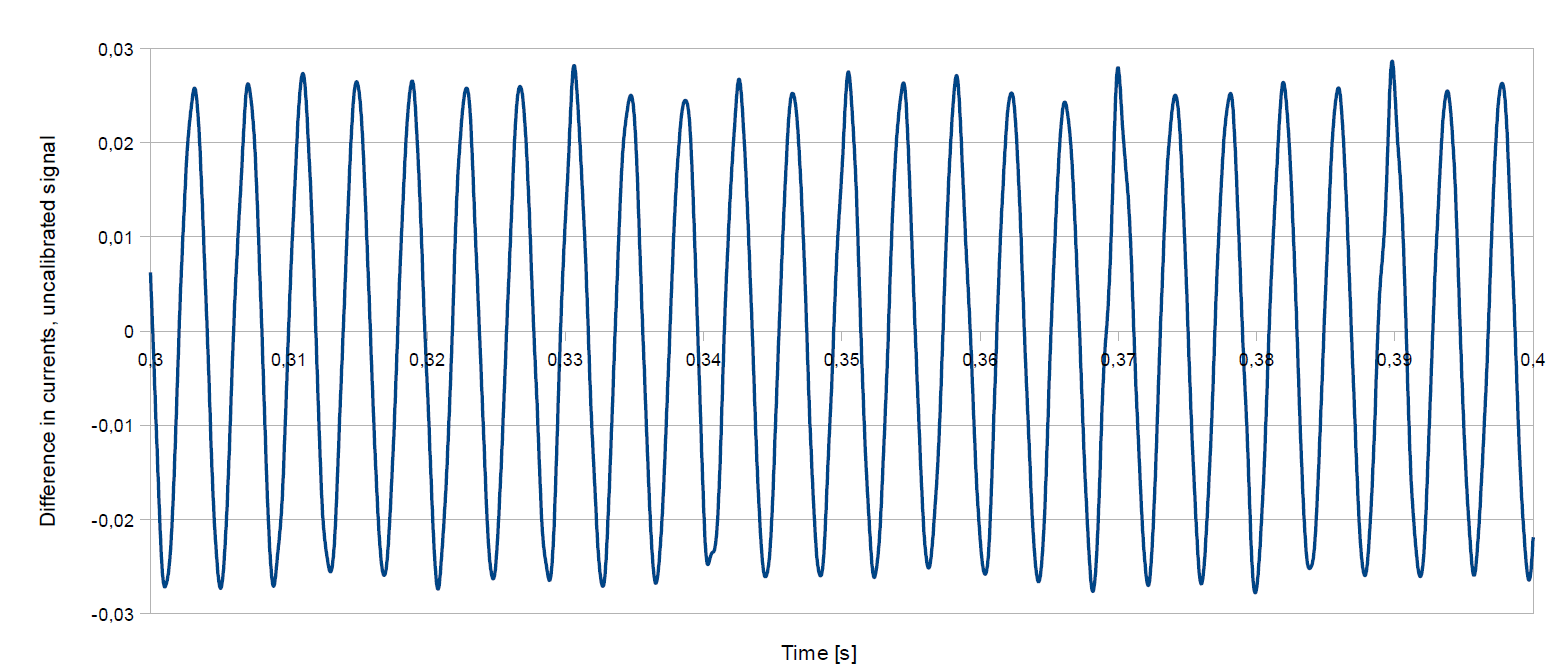
\includegraphics[angle=0,width=0.6\textwidth]{img/frequency}
	\caption{Calibrated amplitude of the oscillations.}
	\label{fig:amplitude}
\end{figure}

Measuring this repeatedly shows that the maximal amplitude highly depends on how hard the tuning fork is stroke, while never exceeding about 0.3 mm and always decreasing in the same way that can me seen in \ref{fig:amplitude}.
	
	\begin{thebibliography}{99}

	\bibitem{FDNotes} \textquotedblleft Solving PDE with Finite difference
	methods,\textquotedblright\ \textit{Lecture notes to Numerical methods for partial differential 	equations}, Umeå University.
	\end{thebibliography}

%	% här brjar alla bilagor. Denna måste finnas med även om bara
%	% bilagor anges i \begin{appendices} ... \end{appendices}
%	\appendix
%
%	\Section{Bilaga 1}
%	\ldots{}ligger direkt i dokumentet
%
%	% bilagor, t.ex. källkod. En tom extrasida kommer att skrivas ut för
%	% att få alla sidnummer att stämma
%	\begin{appendices}
%		\appitem{Källkod}{0}
%		\appsubitem{\texttt{mish.c}}{2}
%		\appsubitem{\texttt{mish.h}}{1}
%		\appitem{En bilaga på 3 sidor}{3}
%	\end{appendices}

\end{document}


% Lite information om hur man arbetar med LaTeX
%-----------------------------------------------
%
% LaTeX-koden kan skrivas med en godtycklig editor.
% Fr att "kompilera" dokumentet anvnds kommandot latex:
%    bergner@peppar:~/edu/sysprog/lab1> latex rapportmall.tex
% Resultatet blir ett antal filer, bl.a. en som heter rapportmall.dvi.
% Denna fil kan anvndas fr att titta hur dokumentet egentligen ser
% ut med hjlp av programmet xdvi:
%    bergner@peppar:~/edu/sysprog/lab1> xdvi rapportmall.dvi &
% Du fr d upp ett fnster som visar ditt dokument. Detta fnster
% kommer automatiskt att uppdateras d du ndrar och kompilerar om din
% LaTeX-kod. 
% Nr du anser att din rapport r frdig att skrivas ut anvnder man
% lmpligtvis kommandona dvips och lpr:
%    bergner@peppar:~/edu/sysprog/lab1> dvips -P ma436ps rapportmall.dvi
% Om man vill ha kvar PostScript-filen som dvips genererar kan man gra:
%    bergner@peppar:~/edu/sysprog/lab1> dvips -o rapport.ps rapportmall.dvi
%    bergner@peppar:~/edu/sysprog/lab1> lpr -P ma436ps rapport.ps
% OBS!!! Fr att innehllsfrteckningen och eventuella referenser till
% tabeller och figurer garanterat ska stmma mste man kra latex 2ggr
% p sitt dokument efter att man har ndrat ngot.
%
%
% Lite information om saker man kan tnkas behva i sitt arbete med LaTeX
%-------------------------------------------------------------------------
%
% FORMATTERA TEXT
%
% Fr att formattera text p lite olika stt kan man anvnda fljande LaTeX-
% kommandon:
%    \textbf{denna text kommer att vara i fetstil}
%    \emph{denna text r viktig (kursiv stil)}
%    \texttt{i denna text blir alla tecken lika breda, som med en skrivmaskin}
%    \textsf{denna text visas med ett typsnitt utan serifer}
%
%
% MATEMATISKA FORMLER
%
% Fr att typstta matematiska formler kan man anvnda:
%    $f(x) = x^2 - 3$, vilket lgger in formeln i texten, eller
%    \begin{displaymath}
%        g(x) = \frac{\sin x}{x}
%    \end{displaymath}, vilket lter formeln visas centrerat p en egen rad
% Om du vill att en formel ska numreras byter du ut displaymath mot equation.
% Det finns massor med matematiska symboler, vilket gr att man behver
% ngon liten manual att titta i om man ska konstruera avancerade formler.
% Se slutet p filen fr lite rd om var du kan hitta sdana.
%
%
% INFOGA FIGURER
%
% Fr att infoga en figur kan man gra p fljande stt:
%    \begin{figure}[htb]
%        \includegraphics[scale=0.5, angle=90]{exec_flow.eps}
%        \caption{Detta r bildtexten}
%        \label{EXECFLOW}
%    \end{figure}
% Om man vill referera till denna bild i texten skulle man d skriva enligt:
%    ...i figur \ref{EXECFLOW} kan man se att...
% Ngra sm frklaringar till figurer:
%    [htb] = talar om hur latex ska frska placera bilden (Here, Top, Bottom)
%            Om du anvnder [!h], innebr det Here!!!
%    scale = kan skala om bilden, om den r skalbar
%    angle = kan rotera bilden
%    exec_flow.eps = filnamnet p bilden. Notera att formatet .EPS anvnds
% Fr att skapa figurer anvnds lmpligtvis programmet xfig:
%    bergner@peppar:~/edu/sysprog/lab1> xfig &
% Rita (och spara ofta) tills du r klar. Vlj sedan "Export" och exportera
% din figur till EPS-format.
% Om man vill kan man anvnda endast \includegraphics, men det r inte ofta
% man gr det.
%
%
% INFOGA TABELLER
%
% Om man vill skapa en tabell gr man p fljande stt:
%    \begin{table}[htb]
%        \begin{tabular}{|rlp{10cm}|}
%            \hline
%            13 & $17.26$ & En kommentar som kan strcka sig ver flera rader \\
%            \hline
%        \end{tabular}
%        \caption{Tabelltexten...}
%        \label{TBL:MINTABELL}
%    \end{table}
% Om man vill kan man endast anvnda raderna 2-6, dvs f en tabell utan text
% och nummer. Om man gr p detta vis kommer tabellen alltid att lggas p
% det stlle den skrivs i koden, dvs ungefr samma sak som [!h] -> Here!!!
% Ngra frklaringar:
%    l, r, c = vnsterjustera, hgerjustera eller centrera kolumn
%    p{bredd} = skapa en vnsterjusterad kolumn med en viss bredd
%               kan innehlla flera rader text
%    | = en vertikal linje i tabellen
%    \hline = en horisontell linje i tabellen
%    & = kolumnseparator
%    \\ = radseparator
% Tnk p att tabeller oftast ser bttre ut med ganska f linjer.
%
%
% INFOGA KLLKOD ELLER UTDATA FRN TESTKRNINGAR
%
% Om man vill infoga kllkod eller ngot annat liknande, t.ex. utdata frn
% en testkrning r det bra om LaTeX terger utdatan korrekt, dvs en radbrytning
% betyder en radbrytning och 8 mellanslag p rad betyder 8 mellanslag p rad.
% Fr att stadkomma detta anvnds:
%    \begin{verbatim}
%        allt som skrivs hr terges exakt, med skrivmaskinstypsnitt
%    \end{verbatim}
% Oftast finns det dock bttre verktyg fr att skriva ut kllkod. Exempel p
% sdana r a2ps, enscript och atp.
%
%
% NDRA STORLEK P TEXT
%
% Om du vill ndra storleken p ett stycke, t.ex. p din nyss infogade
% testkrning omger du stycket med \begin{STORLEK} \end{STORLEK}, dr
% STORLEK r ngon av:
%    tiny, scriptsize, footnotesize, small, normalsize, large, Large,
%    LARGE, huge, Huge
% Tnk p att inte mixtra fr mycket med storlekar bara.
%
%
% SKAPA LISTOR AV OLIKA SLAG
%
% Det r ganska vanligt att man vill rada upp saker p ngot stt. Fr att
% skapa punktlistor anvnds:
%    \begin{itemize}
%        \item Detta r frsta punkten
%        \item Detta r andra punkten
%    \end{itemize}
% Om man istllet vill ha en numrerad lista kan man anvnda enumerate istllet
% fr itemize. Listor kan anvndas i flera niver
%
%
% MER INFORMATION OM LaTeX
%
% Lite blandad information om LaTeX, lnkar och annat hittar du p
% http://www.cs.umu.se/~bergner/latex.htm
% En del information om rapportskrivning hittar du p
% http://www.cs.umu.se/~bergner/rapport/
% Det finns massor med information om LaTeX p Internet. Ett litet urval:
% http://www.giss.nasa.gov/latex/
%     r en mycket vlfylld sida om LaTeX
% http://wwwinfo.cern.ch/asdoc/WWW/essential/essential.html
%     r en manual som genererats utifrn ett LaTeX-dokument mha latex2html
% http://tex.loria.fr/english/
%     r ett fylligt arkiv av lnkar till LaTeX-dokument p Internet
%
% Min personliga favorit r dock manualen "The Not So Short Introduction to
% LaTeX2e", som finns i DVI-format p ~bergner/LaTeX/lshort2e.dvi
% Dr str i princip allt man behver veta. Det r bara att anvnda xdvi och
% titta efter det du sker, vilket oftast finns dr.
% Om du, precis som jag, vill kunna leka med mnga kommandon i LaTeX finns en
% "LaTeX Command Summary" p ~bergner/LaTeX/latexcmds.ps
